\documentclass[10pt,]{article}
\usepackage{lmodern}
\usepackage{amssymb,amsmath}
\usepackage{ifxetex,ifluatex}
\usepackage{fixltx2e} % provides \textsubscript
\ifnum 0\ifxetex 1\fi\ifluatex 1\fi=0 % if pdftex
  \usepackage[T1]{fontenc}
  \usepackage[utf8]{inputenc}
\else % if luatex or xelatex
  \ifxetex
    \usepackage{mathspec}
  \else
    \usepackage{fontspec}
  \fi
  \defaultfontfeatures{Ligatures=TeX,Scale=MatchLowercase}
\fi
% use upquote if available, for straight quotes in verbatim environments
\IfFileExists{upquote.sty}{\usepackage{upquote}}{}
% use microtype if available
\IfFileExists{microtype.sty}{%
\usepackage{microtype}
\UseMicrotypeSet[protrusion]{basicmath} % disable protrusion for tt fonts
}{}
\usepackage[margin=1in]{geometry}
\usepackage{hyperref}
\hypersetup{unicode=true,
            pdftitle={Supplementary for intePareto: An R package for integrative analysis of RNA-Seq and ChIP-Seq data},
            pdfauthor={Yingying Cao, Simo Kitanovski, Daniel Hoffmann},
            pdfborder={0 0 0},
            breaklinks=true}
\urlstyle{same}  % don't use monospace font for urls
\usepackage{biblatex}

\addbibresource{./reference.bib}
\usepackage{color}
\usepackage{fancyvrb}
\newcommand{\VerbBar}{|}
\newcommand{\VERB}{\Verb[commandchars=\\\{\}]}
\DefineVerbatimEnvironment{Highlighting}{Verbatim}{commandchars=\\\{\}}
% Add ',fontsize=\small' for more characters per line
\usepackage{framed}
\definecolor{shadecolor}{RGB}{248,248,248}
\newenvironment{Shaded}{\begin{snugshade}}{\end{snugshade}}
\newcommand{\AlertTok}[1]{\textcolor[rgb]{0.94,0.16,0.16}{#1}}
\newcommand{\AnnotationTok}[1]{\textcolor[rgb]{0.56,0.35,0.01}{\textbf{\textit{#1}}}}
\newcommand{\AttributeTok}[1]{\textcolor[rgb]{0.77,0.63,0.00}{#1}}
\newcommand{\BaseNTok}[1]{\textcolor[rgb]{0.00,0.00,0.81}{#1}}
\newcommand{\BuiltInTok}[1]{#1}
\newcommand{\CharTok}[1]{\textcolor[rgb]{0.31,0.60,0.02}{#1}}
\newcommand{\CommentTok}[1]{\textcolor[rgb]{0.56,0.35,0.01}{\textit{#1}}}
\newcommand{\CommentVarTok}[1]{\textcolor[rgb]{0.56,0.35,0.01}{\textbf{\textit{#1}}}}
\newcommand{\ConstantTok}[1]{\textcolor[rgb]{0.00,0.00,0.00}{#1}}
\newcommand{\ControlFlowTok}[1]{\textcolor[rgb]{0.13,0.29,0.53}{\textbf{#1}}}
\newcommand{\DataTypeTok}[1]{\textcolor[rgb]{0.13,0.29,0.53}{#1}}
\newcommand{\DecValTok}[1]{\textcolor[rgb]{0.00,0.00,0.81}{#1}}
\newcommand{\DocumentationTok}[1]{\textcolor[rgb]{0.56,0.35,0.01}{\textbf{\textit{#1}}}}
\newcommand{\ErrorTok}[1]{\textcolor[rgb]{0.64,0.00,0.00}{\textbf{#1}}}
\newcommand{\ExtensionTok}[1]{#1}
\newcommand{\FloatTok}[1]{\textcolor[rgb]{0.00,0.00,0.81}{#1}}
\newcommand{\FunctionTok}[1]{\textcolor[rgb]{0.00,0.00,0.00}{#1}}
\newcommand{\ImportTok}[1]{#1}
\newcommand{\InformationTok}[1]{\textcolor[rgb]{0.56,0.35,0.01}{\textbf{\textit{#1}}}}
\newcommand{\KeywordTok}[1]{\textcolor[rgb]{0.13,0.29,0.53}{\textbf{#1}}}
\newcommand{\NormalTok}[1]{#1}
\newcommand{\OperatorTok}[1]{\textcolor[rgb]{0.81,0.36,0.00}{\textbf{#1}}}
\newcommand{\OtherTok}[1]{\textcolor[rgb]{0.56,0.35,0.01}{#1}}
\newcommand{\PreprocessorTok}[1]{\textcolor[rgb]{0.56,0.35,0.01}{\textit{#1}}}
\newcommand{\RegionMarkerTok}[1]{#1}
\newcommand{\SpecialCharTok}[1]{\textcolor[rgb]{0.00,0.00,0.00}{#1}}
\newcommand{\SpecialStringTok}[1]{\textcolor[rgb]{0.31,0.60,0.02}{#1}}
\newcommand{\StringTok}[1]{\textcolor[rgb]{0.31,0.60,0.02}{#1}}
\newcommand{\VariableTok}[1]{\textcolor[rgb]{0.00,0.00,0.00}{#1}}
\newcommand{\VerbatimStringTok}[1]{\textcolor[rgb]{0.31,0.60,0.02}{#1}}
\newcommand{\WarningTok}[1]{\textcolor[rgb]{0.56,0.35,0.01}{\textbf{\textit{#1}}}}
\usepackage{longtable,booktabs}
\usepackage{graphicx,grffile}
\makeatletter
\def\maxwidth{\ifdim\Gin@nat@width>\linewidth\linewidth\else\Gin@nat@width\fi}
\def\maxheight{\ifdim\Gin@nat@height>\textheight\textheight\else\Gin@nat@height\fi}
\makeatother
% Scale images if necessary, so that they will not overflow the page
% margins by default, and it is still possible to overwrite the defaults
% using explicit options in \includegraphics[width, height, ...]{}
\setkeys{Gin}{width=\maxwidth,height=\maxheight,keepaspectratio}
\IfFileExists{parskip.sty}{%
\usepackage{parskip}
}{% else
\setlength{\parindent}{0pt}
\setlength{\parskip}{6pt plus 2pt minus 1pt}
}
\setlength{\emergencystretch}{3em}  % prevent overfull lines
\providecommand{\tightlist}{%
  \setlength{\itemsep}{0pt}\setlength{\parskip}{0pt}}
\setcounter{secnumdepth}{0}
% Redefines (sub)paragraphs to behave more like sections
\ifx\paragraph\undefined\else
\let\oldparagraph\paragraph
\renewcommand{\paragraph}[1]{\oldparagraph{#1}\mbox{}}
\fi
\ifx\subparagraph\undefined\else
\let\oldsubparagraph\subparagraph
\renewcommand{\subparagraph}[1]{\oldsubparagraph{#1}\mbox{}}
\fi

%%% Use protect on footnotes to avoid problems with footnotes in titles
\let\rmarkdownfootnote\footnote%
\def\footnote{\protect\rmarkdownfootnote}

%%% Change title format to be more compact
\usepackage{titling}

% Create subtitle command for use in maketitle
\providecommand{\subtitle}[1]{
  \posttitle{
    \begin{center}\large#1\end{center}
    }
}

\setlength{\droptitle}{-2em}

  \title{Supplementary for intePareto: An R package for integrative analysis of
RNA-Seq and ChIP-Seq data}
    \pretitle{\vspace{\droptitle}\centering\huge}
  \posttitle{\par}
    \author{Yingying Cao, Simo Kitanovski, Daniel Hoffmann}
    \preauthor{\centering\large\emph}
  \postauthor{\par}
    \date{}
    \predate{}\postdate{}
  

\begin{document}
\maketitle

A frequent question in biology is: How do the functions of different
cell types differ? E.g.~we may be interested in what the effect of a
mutation or gene knockout is in terms of functional differences between
wild type and mutant/knockout, or how cellular function changes between
two developmental stages of a cell type. One way of understanding such
functional difference is to characterize them at the level of
differences in repertoires in active genes or suppressed genes. The
characterization of differential gene expression is helpful in this
respect, but even more expressive is the combination of evidence from
different experiments, namely measurements of gene expression (RNA-Seq)
and measurements of various histone modifications (ChIP-Seq) that allow
assessment of activation or suppression state of genes. In our
experience, this combination of information gives a clearer picture of
the cellular function at the molecular level than using any of the
information types alone.

We have therefore developed the R package intePareto that allows such a
combination of different types of sequencing data. The intePareto
workflow starts with RNA-Seq and ChIP-Seq data for two different cell
types or conditions. The ChIP-Seq data will in general comprise
information on several histone modifications with activating or
repressing function. The end product of intePareto is a list of genes
prioritized according to congruence of changes of gene expression and
histone modifications.

In the following we demonstrate the technical workflow with the
published dataset GSE48519 where a Tet2 knockout cell line is compared
to the wild type \autocite{hon2014}. The raw data were downloaded from
Gene Expression Omnibus. This set contains 4 RNA-Seq samples, 31
ChIP-Seq samples with histone modification mark of H3K4me1, H3K4me3,
H3K9me3, H3K27ac, H3K27me3, H3K36me3 and control for Tet2 knockout and
wild type mouse embryonic stem cells (mESCs) separately.

\hypertarget{preprocessing-of-rna-seq-data-and-chip-seq-data}{%
\subsubsection{Preprocessing of RNA-Seq data and ChIP-Seq
data}\label{preprocessing-of-rna-seq-data-and-chip-seq-data}}

The quality of the fastq data was examined with FastQC \autocite{andrews2010fastqc}. The RNA-Seq data was then preprocessed by Kallisto \autocite{bray2016},
and ChIP-Seq data was preprocessed by BWA \autocite{li2009a}, Samtools
\autocite{li2009}. The meta data below gives an overview of the
preprocessed files that are the input files for intePareto.

\begin{Shaded}
\begin{Highlighting}[]
\KeywordTok{library}\NormalTok{(intePareto)}
\end{Highlighting}
\end{Shaded}

\begin{Shaded}
\begin{Highlighting}[]
\NormalTok{rna_meta}
\end{Highlighting}
\end{Shaded}

\begin{verbatim}
##         SRR condition                                              files
## 1 SRR925874 wild.type ./data/tet2/kallisto/outputSRR925874/abundance.tsv
## 2 SRR925875 wild.type ./data/tet2/kallisto/outputSRR925875/abundance.tsv
## 5 SRR925878  tet2.out ./data/tet2/kallisto/outputSRR925878/abundance.tsv
## 6 SRR925879  tet2.out ./data/tet2/kallisto/outputSRR925879/abundance.tsv
\end{verbatim}

\begin{Shaded}
\begin{Highlighting}[]
\NormalTok{chip_meta[}\DecValTok{1}\OperatorTok{:}\DecValTok{2}\NormalTok{,]}
\end{Highlighting}
\end{Shaded}

\begin{verbatim}
##         SRR    mark condition                                   files
## 1 SRR925639 H3K4me1 wild.type ./data/tet2/output/SRR925639_sorted.bam
## 2 SRR925640 H3K4me3 wild.type ./data/tet2/output/SRR925640_sorted.bam
\end{verbatim}

\hypertarget{match-match-rna-seq-and-chip-seq-data-on-the-gene-level}{%
\subsubsection{\texorpdfstring{1. \textbf{match}: Match RNA-Seq and
ChIP-Seq data on the gene
level}{1. match: Match RNA-Seq and ChIP-Seq data on the gene level}}\label{match-match-rna-seq-and-chip-seq-data-on-the-gene-level}}

Take the meta data of the preprocessed RNA-Seq and ChIP-Seq data as
input. The first step of intePareto is to match the RNA-Seq data and
ChIP-Seq data on the gene level. There are two strategies available now
to do the matching step: (1) highest - choose the maximum promoter
abundance value among all the promoters as a representative of the
ChIP-Seq signal for this gene. (2) weighted.mean - calculate the
weighted mean of the abundance value of all the promoters to represent
the ChIP-Seq signal for this gene. Here we choose ``highest'':

\begin{Shaded}
\begin{Highlighting}[]
\KeywordTok{library}\NormalTok{(intePareto)}
\NormalTok{chip_meta_noH3K36me3 <-}\StringTok{ }\NormalTok{chip_meta[}\OperatorTok{!}\NormalTok{chip_meta}\OperatorTok{$}\NormalTok{mark}\OperatorTok\StringTok{"H3K36me3"}\NormalTok{,]}
\NormalTok{res}\FloatTok{.1}\NormalTok{ <-}\StringTok{ }\KeywordTok{doMatch}\NormalTok{(}\DataTypeTok{rnaMeta =}\NormalTok{ rna_meta, }\CommentTok{# metadata of RNA-Seq}
                 \DataTypeTok{chipMeta =}\NormalTok{ chip_meta_noH3K36me3, }\CommentTok{# metadata or ChIP-Seq}
                 \DataTypeTok{region =} \StringTok{"promoter"}\NormalTok{, }\CommentTok{# specify the region}
                 \DataTypeTok{method =} \StringTok{"highest"}\NormalTok{, }\CommentTok{# specify the strategy to do the match}
                 \DataTypeTok{ensemblDataset =} \StringTok{"mmusculus_gene_ensembl"} 
                 \CommentTok{# specify the dataset of corresponing species}
\NormalTok{)}
\NormalTok{chip_meta_H3K36me3 <-}\StringTok{ }\NormalTok{chip_meta[chip_meta}\OperatorTok{$}\NormalTok{mark}\OperatorTok\StringTok{"H3K36me3"}\NormalTok{,]}

\NormalTok{res}\FloatTok{.2}\NormalTok{ <-}\StringTok{ }\KeywordTok{doMatch}\NormalTok{(}\DataTypeTok{rnaMeta =}\NormalTok{ rna_meta, }\CommentTok{# metadata of RNA-Seq}
                 \DataTypeTok{chipMeta =}\NormalTok{ chip_meta_H3K36me3, }\CommentTok{# metadata or ChIP-Seq}
                 \DataTypeTok{method =} \StringTok{"highest"}\NormalTok{, }\CommentTok{# we don't need this parameter if we choose }
                 \CommentTok{# genebody, but it doesn't matter if we choose}
                 \DataTypeTok{region =} \StringTok{"genebody"}\NormalTok{, }\CommentTok{# specify the region}
                 \DataTypeTok{ensemblDataset =} \StringTok{"mmusculus_gene_ensembl"} 
                 \CommentTok{# specify the dataset of corresponing species}
\NormalTok{)}
\NormalTok{res}\FloatTok{.1}\OperatorTok{$}\NormalTok{matched.data <-}\StringTok{ }\KeywordTok{merge}\NormalTok{(res}\FloatTok{.1}\OperatorTok{$}\NormalTok{matched.data,}
\NormalTok{                            res}\FloatTok{.2}\OperatorTok{$}\NormalTok{matched.data)}
\NormalTok{res}\FloatTok{.1}\OperatorTok{$}\NormalTok{res.chip <-}\StringTok{ }\KeywordTok{merge}\NormalTok{(res}\FloatTok{.1}\OperatorTok{$}\NormalTok{res.chip,}
\NormalTok{                        res}\FloatTok{.2}\OperatorTok{$}\NormalTok{res.chip)}
\NormalTok{res <-}\StringTok{ }\NormalTok{res}\FloatTok{.1}
\end{Highlighting}
\end{Shaded}

Figure 1 shows the correlation matrix, the color represents the value of
correlation coefficients of Spearman's rank correlation of all samples.
From this figure we can see that RNA-Seq (wild.type\_REP1,
wild.type\_REP2, tet2.out\_REP1, tet2.out\_REP2) positively correlate
with active histone modification markers (H3K4me3, H3K27ac, H3K4me1, and
H3K36me3), and negatively correlate with repressive histone modification
markers (H3K27me3 and H3K9me3). This can confirm our match strategy
works well for the match of RNA-Seq and ChIP-Seq data on the gene level.

\begin{figure}
\centering
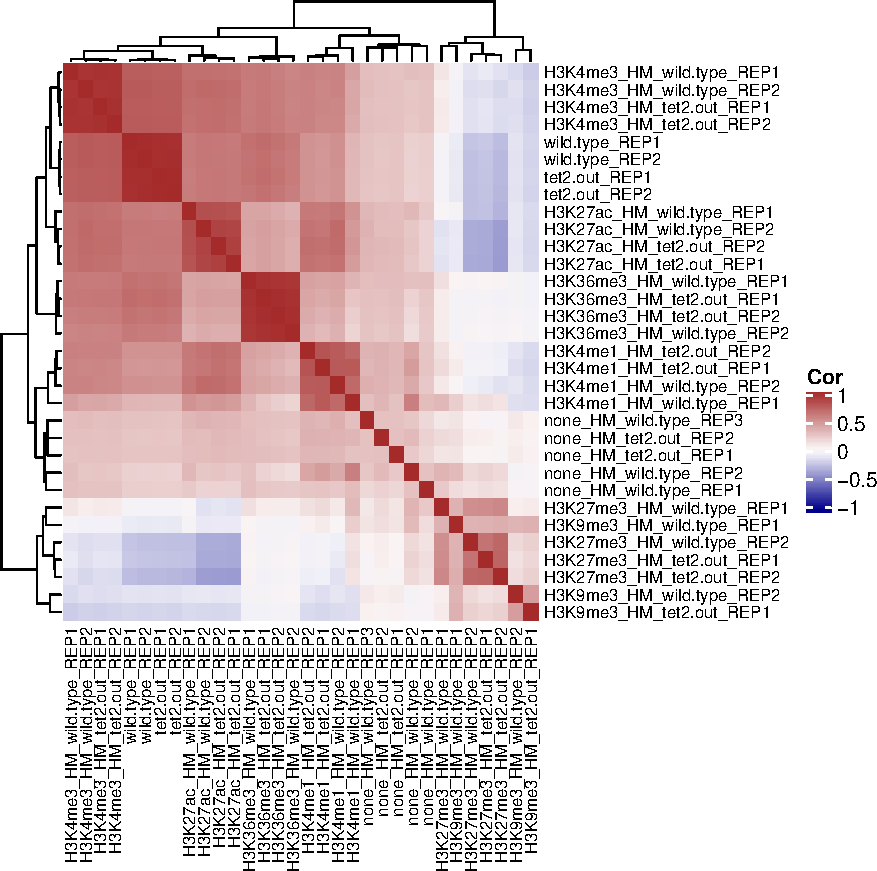
\includegraphics{supplement_file_files/figure-latex/unnamed-chunk-9-1.pdf}
\caption{Correlation of RNA-Seq and ChIP-Seq}
\end{figure}

\newpage

\hypertarget{integration-integrate-rna-seq-and-chip-seq-data-by-calculating-logfoldchange-and-z-scores}{%
\subsubsection{\texorpdfstring{2. \textbf{integration}: Integrate
RNA-Seq and ChIP-Seq data by calculating logFoldChange and Z
scores}{2. integration: Integrate RNA-Seq and ChIP-Seq data by calculating logFoldChange and Z scores}}\label{integration-integrate-rna-seq-and-chip-seq-data-by-calculating-logfoldchange-and-z-scores}}

After the match of RNA-Seq and ChIP-Seq at the gene level, the
integration of these two types of data is conducted through the
\textbf{doIntegration} function by calculating logFoldChange of RNA-Seq
and ChIP-Seq and then calculate Z scores for each marker. The input of
the function is a list result from \textbf{doMatch} function.

\begin{Shaded}
\begin{Highlighting}[]
\NormalTok{df_final <-}\StringTok{ }\KeywordTok{doIntegration}\NormalTok{(}\DataTypeTok{res =}\NormalTok{ res, }\CommentTok{# result list from "doMatch" function}
                          \DataTypeTok{type =} \StringTok{"apeglm"}\NormalTok{, }\CommentTok{# shrinkage estimator, default is "apeglm"}
                          \DataTypeTok{ref =} \StringTok{"wild.type"}\NormalTok{, }\CommentTok{# specifying the reference level}
                          \DataTypeTok{apeAdapt =} \OtherTok{FALSE}\NormalTok{)}
\end{Highlighting}
\end{Shaded}

The result of the second step from \textbf{doIntegration} function
contains the logFoldChange of RNA-Seq and ChIP-Seq as well as the Z
score of each mark for each gene (shown as the table below).

\begin{longtable}[]{@{}lrrrrrrr@{}}
\caption{integration results}\tabularnewline
\toprule
& z.H3K9me3 & z.none & z.H3K27me3 & z.H3K27ac & z.H3K4me3 & z.H3K4me1 &
z.H3K36me3\tabularnewline
\midrule
\endfirsthead
\toprule
& z.H3K9me3 & z.none & z.H3K27me3 & z.H3K27ac & z.H3K4me3 & z.H3K4me1 &
z.H3K36me3\tabularnewline
\midrule
\endhead
0610009B22Rik & 1.5096313 & -0.4556445 & 1.1294972 & -0.0600427 &
0.1922781 & -0.3990826 & 0.1116033\tabularnewline
0610010F05Rik & 0.0727513 & -0.3159894 & 0.1848376 & 1.2379816 &
-0.3030021 & 0.1750952 & -0.1077852\tabularnewline
0610010K14Rik & 0.2818030 & 0.5665779 & 0.3684958 & 0.1205920 &
0.0840617 & 0.0560468 & 0.0950096\tabularnewline
0610012G03Rik & -0.0402419 & -0.0577281 & -0.0344298 & 0.0053385 &
0.0248794 & 0.0119307 & -0.0709771\tabularnewline
0610030E20Rik & -0.2843424 & -0.0069848 & -0.0345165 & 0.5311879 &
-0.1859840 & -0.0157660 & -0.1489075\tabularnewline
0610040J01Rik & 0.0263985 & -0.6136573 & 0.0738724 & 1.2450397 &
0.0459432 & -0.0293661 & 0.3395275\tabularnewline
1110002E22Rik & -0.1117175 & -0.6161363 & 0.3220724 & -0.0374538 &
0.0682505 & -0.4427649 & 0.4736603\tabularnewline
1110004F10Rik & -0.0075126 & 0.0382641 & -0.0531325 & -0.0302648 &
0.0218445 & 0.0215032 & 0.0285630\tabularnewline
1110008P14Rik & 0.5878211 & 0.1613085 & -0.0158789 & -0.0216326 &
-0.1131650 & 0.1088885 & 0.2975963\tabularnewline
1110012L19Rik & -0.7605611 & -0.2186961 & -0.4329753 & -0.3474599 &
-0.1035559 & -0.2430795 & 0.3229549\tabularnewline
1110017D15Rik & -0.5635032 & -0.0215326 & 0.1116994 & -0.2396299 &
0.2999805 & 0.4402020 & -0.2901453\tabularnewline
1110032A03Rik & -0.0308223 & 1.3990756 & -0.3721691 & 0.5582615 &
-0.7094221 & -0.9638899 & 0.4072242\tabularnewline
1110032F04Rik & -0.0619083 & 0.2234994 & -0.0579622 & 0.1148733 &
0.0706187 & 0.1086061 & 0.1350982\tabularnewline
1110051M20Rik & 0.0778253 & -0.0865843 & -0.2830442 & -0.1500254 &
0.1005083 & -0.2821450 & 0.0665700\tabularnewline
1110059E24Rik & -0.0749205 & -0.1335756 & 0.0250346 & 0.2520036 &
-0.1724477 & -0.2854025 & -0.1534097\tabularnewline
\bottomrule
\end{longtable}

\newpage

\hypertarget{prioritization-prioritization-of-genes-based-on-z-scores-with-pareto-optimization}{%
\subsubsection{\texorpdfstring{3. \textbf{prioritization}:
prioritization of genes based on Z scores with Pareto
optimization}{3. prioritization: prioritization of genes based on Z scores with Pareto optimization}}\label{prioritization-prioritization-of-genes-based-on-z-scores-with-pareto-optimization}}

Take the Z scores of several different histone modifications as input,
the prioritization of genes based on Z scores can be formulated as
multiobjective optimization problem and solved with Pareto optimization
\autocite{ngatchou2005}. The aim of Pareto optimization method is to
find the Pareto optimal trade-off (Pareto front) between conflicting
objectives (such as minimizing Z score of H3K27me3 and maximizing
z-score of H3K4me3 for each gene). The results of Pareto optimization
method is a rank-ordering of the genes by the level of the congruent
changes in RNA-Seq and ChIP-Seq (shown as table below).

\begin{Shaded}
\begin{Highlighting}[]
\NormalTok{nr.fronts <-}\StringTok{ }\DecValTok{50} \CommentTok{# choose a large number to include all the fronts}
\NormalTok{objective <-}\StringTok{ }\KeywordTok{data.frame}\NormalTok{(}\DataTypeTok{mark =} \KeywordTok{c}\NormalTok{(}\StringTok{"z.H3K27ac"}\NormalTok{, }\StringTok{"z.H3K4me3"}\NormalTok{, }\StringTok{"z.H3K4me1"}\NormalTok{,}
                                 \StringTok{"z.H3K36me3"}\NormalTok{, }\StringTok{"z.H3K9me3"}\NormalTok{, }\StringTok{"z.H3K27me3"}\NormalTok{), }
                        \DataTypeTok{obj=}\KeywordTok{c}\NormalTok{(}\StringTok{"max"}\NormalTok{,}\StringTok{"max"}\NormalTok{,}\StringTok{"max"}\NormalTok{,}\StringTok{"max"}\NormalTok{,}\StringTok{"min"}\NormalTok{,}\StringTok{"min"}\NormalTok{),}
                        \DataTypeTok{stringsAsFactors=}\OtherTok{FALSE}\NormalTok{)}
\NormalTok{res_final <-}\StringTok{ }\KeywordTok{doPareto}\NormalTok{(}\DataTypeTok{df_final =}\NormalTok{ df_final, }
                      \DataTypeTok{objective =}\NormalTok{ objective, }
                      \DataTypeTok{nr.fronts =}\NormalTok{ nr.fronts)}
\end{Highlighting}
\end{Shaded}

\begin{longtable}[]{@{}lrrrrrrrr@{}}
\caption{prioritization results}\tabularnewline
\toprule
& z.H3K9me3 & z.none & z.H3K27me3 & z.H3K27ac & z.H3K4me3 & z.H3K4me1 &
z.H3K36me3 & front\tabularnewline
\midrule
\endfirsthead
\toprule
& z.H3K9me3 & z.none & z.H3K27me3 & z.H3K27ac & z.H3K4me3 & z.H3K4me1 &
z.H3K36me3 & front\tabularnewline
\midrule
\endhead
Atp6v0c-ps2 & 16.589667 & 3.2706193 & -20.013204 & -1.725424 &
11.8417083 & -0.5113998 & 10.440533 & 1\tabularnewline
Catsperg1 & -8.061640 & -1.5505929 & 1.034593 & 10.164148 & 12.7109471 &
0.8538197 & 12.002940 & 1\tabularnewline
Fam110c & 7.090283 & 4.5737313 & -3.192932 & 38.702950 & 7.4691643 &
4.8392381 & 12.702844 & 1\tabularnewline
Grb14 & -3.354402 & 2.4001542 & -14.829860 & 27.547845 & 10.8787232 &
4.9987109 & 15.616601 & 1\tabularnewline
Khdc1a & -9.654657 & -5.3475747 & 3.041933 & 17.776863 & 11.8376748 &
20.2619271 & 14.673243 & 1\tabularnewline
Metrn & -8.142343 & -6.7852712 & -5.716880 & -10.044830 & 8.9894024 &
11.5985664 & 12.760880 & 1\tabularnewline
Olfr94 & -5.706979 & 0.4598344 & -36.221443 & 99.403578 & 21.5264205 &
20.2764413 & 1.578383 & 1\tabularnewline
Olig1 & -6.158681 & 11.2312845 & -20.694139 & 34.781308 & 20.0243582 &
8.6956798 & 4.906146 & 1\tabularnewline
Pramef17 & 5.581220 & 8.4221983 & -6.412906 & 11.671704 & 6.1742990 &
21.5723380 & 21.153664 & 1\tabularnewline
Trav5-2 & -8.224873 & 2.4279795 & -3.729377 & 23.326949 & -0.1153585 &
13.0210337 & 18.820450 & 1\tabularnewline
Trim34b & -10.368544 & -0.9556500 & -14.980885 & 5.767722 & 3.5631355 &
-11.3481747 & -6.496720 & 1\tabularnewline
Tspo2 & -3.858320 & -5.9325064 & -4.143173 & 13.234274 & 30.3344625 &
12.5968673 & 38.445580 & 1\tabularnewline
Ttll11 & -3.243813 & 0.0535220 & 1.956712 & 98.616938 & 7.3652294 &
7.1142097 & 18.991588 & 1\tabularnewline
Ubd & -26.955101 & 8.3544039 & -12.420790 & 73.875377 & 115.7006521 &
42.1527121 & 11.752621 & 1\tabularnewline
Zfp786 & -6.054174 & 2.8041174 & -0.747937 & 6.618457 & 3.1202473 &
7.2548820 & 5.319367 & 2\tabularnewline
\bottomrule
\end{longtable}

\newpage

\hypertarget{compare-our-integrative-results-with-other-approach-and-rna-seq-alone}{%
\subsubsection{Compare our integrative results with other approach and
RNA-Seq
alone}\label{compare-our-integrative-results-with-other-approach-and-rna-seq-alone}}

To evaluate the performance of our method we did the integrative
analysis with a recent published the hierarchical Bayesian model-based
clustering approach (model-based approach )\autocite{Schafer2017} and
analysis of RNA-Seq alone, a functional quality metric, enrichment score
of interesting terms for each data set is used to do comparison research
between our integrative approach, the model-based approach and the
analysis of RNA-Seq data alone. The enrichment score is defined as
\(N(G_i \cap G_r) \mid N(G_r)\), in which \(G_i\) stands for the genes
in the interesting GO terms, \(G_r\) stands for the genes in the result
of analysis.

Both our integrative approach and the model-based approach found that
the genes in the final result or the top rank gene (intePareto) enriched
in ``limb morphogenesis'' GO term {[}Figure 2{]}, which is consist with
results in a recently published research \autocite{li2018}. Our approach
also found genes in the top-ranked list enriched in ``mammary gland
formation'' which is discussed in this review \autocite{holliday2018}.
This result will be hidden when RNA-Seq data alone was analyzed or the
model-based approach was used. When compared to the model-based
approach\autocite{schafer2017}, our method outperformed it by having
comparable results at the top genes and offering more informative
results by providing the rank-ordered list of the remaining genes.

\begin{figure}
\centering
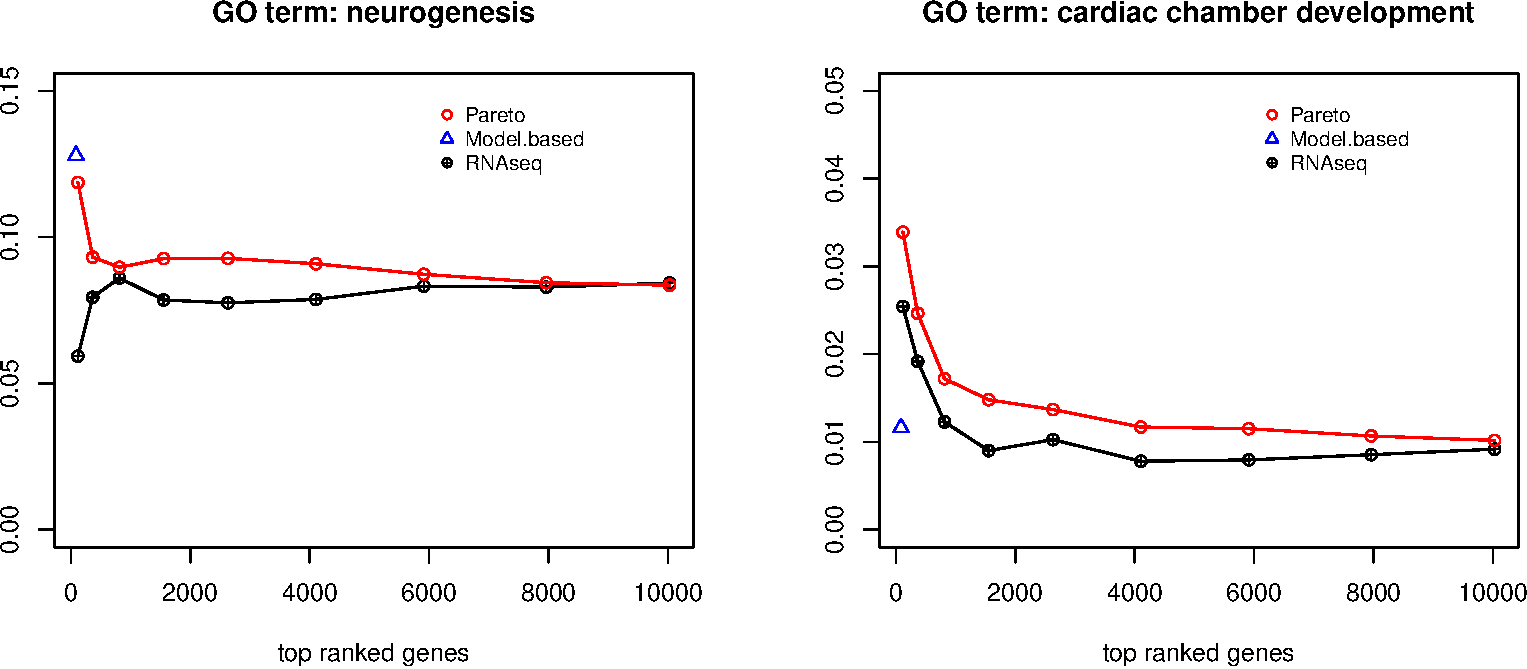
\includegraphics{supplement_file_files/figure-latex/unnamed-chunk-17-1.pdf}
\caption{Compare intePareto with another approach and RNAseq alone}
\end{figure}

\begin{Shaded}
\begin{Highlighting}[]
\KeywordTok{sessionInfo}\NormalTok{()}
\end{Highlighting}
\end{Shaded}

\begin{verbatim}
## R version 3.6.1 (2019-07-05)
## Platform: x86_64-pc-linux-gnu (64-bit)
## Running under: Ubuntu 16.04.6 LTS
## 
## Matrix products: default
## BLAS:   /usr/lib/libblas/libblas.so.3.6.0
## LAPACK: /usr/lib/lapack/liblapack.so.3.6.0
## 
## locale:
##  [1] LC_CTYPE=en_US.UTF-8       LC_NUMERIC=C              
##  [3] LC_TIME=de_DE.UTF-8        LC_COLLATE=en_US.UTF-8    
##  [5] LC_MONETARY=de_DE.UTF-8    LC_MESSAGES=en_US.UTF-8   
##  [7] LC_PAPER=de_DE.UTF-8       LC_NAME=C                 
##  [9] LC_ADDRESS=C               LC_TELEPHONE=C            
## [11] LC_MEASUREMENT=de_DE.UTF-8 LC_IDENTIFICATION=C       
## 
## attached base packages:
## [1] grid      stats     graphics  grDevices utils     datasets  methods  
## [8] base     
## 
## other attached packages:
## [1] knitr_1.24           circlize_0.4.8       ComplexHeatmap_2.0.0
## [4] intePareto_0.1.1     apeglm_1.6.0        
## 
## loaded via a namespace (and not attached):
##   [1] bitops_1.0-6                matrixStats_0.55.0         
##   [3] bit64_0.9-7                 httr_1.4.1                 
##   [5] RColorBrewer_1.1-2          progress_1.2.2             
##   [7] GenomeInfoDb_1.20.0         numDeriv_2016.8-1.1        
##   [9] tools_3.6.1                 backports_1.1.4            
##  [11] R6_2.4.0                    rpart_4.1-15               
##  [13] Hmisc_4.2-0                 DBI_1.1.0                  
##  [15] lazyeval_0.2.2              BiocGenerics_0.30.0        
##  [17] colorspace_1.4-1            GetoptLong_0.1.7           
##  [19] nnet_7.3-12                 prettyunits_1.0.2          
##  [21] tidyselect_1.0.0            gridExtra_2.3              
##  [23] DESeq2_1.24.0               bit_1.1-14                 
##  [25] compiler_3.6.1              Biobase_2.44.0             
##  [27] htmlTable_1.13.1            DelayedArray_0.10.0        
##  [29] scales_1.0.0                checkmate_1.9.4            
##  [31] genefilter_1.66.0           stringr_1.4.0              
##  [33] digest_0.6.20               Rsamtools_2.0.0            
##  [35] foreign_0.8-72              rmarkdown_1.15             
##  [37] XVector_0.24.0              base64enc_0.1-3            
##  [39] pkgconfig_2.0.2             htmltools_0.3.6            
##  [41] highr_0.8                   bbmle_1.0.20               
##  [43] GlobalOptions_0.1.0         htmlwidgets_1.3            
##  [45] rlang_0.4.5                 rstudioapi_0.10            
##  [47] RSQLite_2.1.2               rPref_1.3                  
##  [49] shape_1.4.4                 BiocParallel_1.18.1        
##  [51] acepack_1.4.1               dplyr_0.8.3                
##  [53] RCurl_1.95-4.12             magrittr_1.5               
##  [55] GenomeInfoDbData_1.2.1      Formula_1.2-3              
##  [57] Matrix_1.2-17               Rcpp_1.0.2                 
##  [59] munsell_0.5.0               S4Vectors_0.22.1           
##  [61] stringi_1.4.3               yaml_2.2.0                 
##  [63] MASS_7.3-51.4               SummarizedExperiment_1.14.1
##  [65] zlibbioc_1.30.0             plyr_1.8.4                 
##  [67] blob_1.2.0                  parallel_3.6.1             
##  [69] crayon_1.3.4                lattice_0.20-38            
##  [71] Biostrings_2.52.0           splines_3.6.1              
##  [73] annotate_1.62.0             hms_0.5.1                  
##  [75] locfit_1.5-9.1              pillar_1.4.2               
##  [77] igraph_1.2.4.1              GenomicRanges_1.36.0       
##  [79] rjson_0.2.20                geneplotter_1.62.0         
##  [81] biomaRt_2.40.5              stats4_3.6.1               
##  [83] XML_3.98-1.20               glue_1.3.1                 
##  [85] evaluate_0.14               latticeExtra_0.6-28        
##  [87] data.table_1.12.2           RcppParallel_4.4.3         
##  [89] png_0.1-7                   vctrs_0.2.4                
##  [91] gtable_0.3.0                purrr_0.3.2                
##  [93] clue_0.3-57                 assertthat_0.2.1           
##  [95] ggplot2_3.2.1               emdbook_1.3.11             
##  [97] xfun_0.9                    xtable_1.8-4               
##  [99] coda_0.19-3                 survival_2.44-1.1          
## [101] tibble_2.1.3                GenomicAlignments_1.20.1   
## [103] AnnotationDbi_1.46.1        memoise_1.1.0              
## [105] IRanges_2.18.3              cluster_2.1.0
\end{verbatim}

\printbibliography


\end{document}
